\begin{center}
	\begin{tabular}{M{9.25cm}M{8.75cm}}
		\textbf{TRUNG TÂM MANABIE}& \textbf{ÔN TẬP KIỂM TRA CUỐI HỌC KÌ I}\\
		\textbf{MÃ ĐỀ: 002}& \textbf{Bài thi môn: VẬT LÝ 11}\\
		\textit{(Đề thi có 04 trang)}& \textit{Thời gian làm bài: 50 phút, không kể phát đề}
		
		\noindent\rule{4cm}{0.8pt} \\
	\end{tabular}
\end{center}
\setcounter{section}{0}
\section{Câu trắc nghiệm nhiều phương án lựa chọn}
\textit{Thí sinh trả lời từ câu 1 đến câu 18. Mỗi câu hỏi thí sinh chọn một phương án}
\setcounter{ex}{0}
\Opensolutionfile{ans}[ans/G11-FINAL-SEM1-002-TN]
% ===================================================================
\begin{ex}
	Sóng cơ được gọi là sóng dọc khi các phần tử môi trường dao động theo phương
	\choice
	{nằm ngang}
	{\True trùng với phương truyền sóng}
	{thẳng đứng}
	{vuông góc với phương truyền sóng}
	\loigiai{}
\end{ex}
% ===================================================================
\begin{ex}
Một vật dao động điều hòa. Khi vật đi từ vị trí biên dương đến biên âm thì gia tốc
	\choice
	{giảm rồi tăng}
	{tăng rồi giảm}
	{giảm}
	{\True tăng}
	\loigiai{}
\end{ex}
% ===================================================================
\begin{ex}
Một vật dao động điều hòa với theo phương trình $x=A\cos\left(\omega t+\varphi\right)$ với $A$, $\omega$, $\varphi$ là hằng số thì pha của dao động
	\choice
	{không đổi theo thời gian}
	{biến thiên điều hòa theo thời gian}
	{\True là hàm bậc nhất với thời gian}
	{là hàm bậc hai của thời gian}
	\loigiai{}
\end{ex}
% ===================================================================
\begin{ex}
Một vật dao động điều hòa dọc theo trục $Ox$ với phương trình $x=A\sin \omega t$. Nếu chọn gốc toạ độ O tại vị trí cân bằng của vật thì gốc thời gian $t=0$ là lúc vật
	\choice
	{ở vị trí li độ cực đại thuộc phần dương của trục $Ox$}
	{qua vị trí cân bằng O ngược chiều dương của trục $Ox$}
	{ở vị trí li độ cực đại thuộc phần âm của trục $Ox$}
	{\True qua vị trí cân bằng O theo chiều dương của trục $Ox$}
	\loigiai{}
\end{ex}
% ===================================================================
\begin{ex}
Loại sóng nào sau đây được dùng trong thông tin liên lạc bằng vệ tinh
	\choice
	{\True sóng vô tuyến có bước sóng cực ngắn}
	{vi sóng}
	{sóng vô tuyến có bước sóng trung}
	{sóng siêu âm}
	\loigiai{}
\end{ex}
% ===================================================================
\begin{ex}
Trong sự truyền sóng cơ, tần số dao động của một phần tử môi trường có sóng truyền qua được gọi là
	\choice
	{biên độ của sóng}
	{tốc độ truyền sóng}
	{\True tần số của sóng}
	{năng lượng sóng}
	\loigiai{}
\end{ex}
% ===================================================================
\begin{ex}
Phát biểu nào sau đây đúng khi nói về dao động điều hoà?
	\choice
	{Cơ năng biến thiên tuần hoàn vì động năng biến thiên tuần hoàn}
	{Thế năng biến thiên tuần hoàn nên cơ năng biến thiên tuần hoàn}
	{Cơ năng biến thiên tuần hoàn vì động năng và thế năng biến thiên tuần hoàn}
	{\True Cơ năng luôn không đổi mặc dù động năng và thế năng biến thiên tuần hoàn}
	\loigiai{}
\end{ex}
% ===================================================================
\begin{ex}
Cho một vật dao động điều hòa có phương trình chuyển động $x=10\cos\left(2\pi t-\dfrac{\pi}{6}\right)$. Biên độ dao động của vật là
	\choice
	{\True $\SI{10}{\centi\meter}$}
	{$\SI{20}{\centi\meter}$}
	{$\xsi{20\pi}{\centi\meter}$}
	{$\xsi{10\pi}{\centi\meter}$}
	\loigiai{}
\end{ex}
% ===================================================================
\begin{ex}
Chọn phát biểu \textbf{sai}. Tia hồng ngoại và tia tử ngoại đều có
	\choice
	{trong ánh sáng Mặt Trời}
	{\True tác dụng làm ion hoá không khí}
	{là bức xạ điện từ không thấy được}
	{những ứng dụng trong y học}
	\loigiai{}
\end{ex}
% ===================================================================
\begin{ex}
Tại nơi có gia tốc trọng trường là $g$, một con lắc lò xo treo thẳng đứng đang dao động điều hòa. Biết tại vị trí cân bằng của vật, độ dãn của lò xo là $\Delta\ell$. Chu kì dao động của con lắc này là
	\choice
	{$T=\dfrac{1}{2\pi}\sqrt{\dfrac{\Delta\ell}{g}}$}
	{$T=2\pi\sqrt{\dfrac{\Delta\ell}{g}}$}
	{$T=\dfrac{1}{2\pi}\sqrt{\dfrac{g}{\Delta\ell}}$}
	{\True $T=2\pi\sqrt{\dfrac{g}{\Delta\ell}}$}
	\loigiai{}
\end{ex}
% ===================================================================
\begin{ex}
Một vật dao động điều hòa theo trục $Ox$, với vị trí cân bằng là gốc tọa độ. Gia tốc của vật phụ thuộc vào li độ theo phương trình $a=–400\pi^2 x$. Số dao động toàn phần mà vật thực hiện trong mỗi giây là
	\choice
	{20}
	{\True 10}
	{40}
	{5}
	\loigiai{}
\end{ex}
% ===================================================================
\begin{ex}
\immini{Một vật có khối lượng $\SI{1}{\kilogram}$ dao động điều hòa xung quanh vị trí cân bằng. Đồ thị thế năng của vật theo thời gian được cho như hình vẽ. Lấy $\pi^2=10$. Biên độ dao động của vật là
	\choice
	{$\SI{60}{\centi\meter}$}
	{$\SI{3.75}{\centi\meter}$}
	{\True $\SI{15}{\centi\meter}$}
	{$\SI{30}{\centi\meter}$}}
	{\vspace{-0.5cm}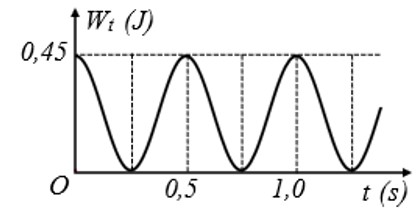
\includegraphics[scale=0.7]{../figs/G11-FINAL-SEM1-002-1}}
	\loigiai{}
\end{ex}
% ===================================================================
\begin{ex}
Một sóng cơ hình sin truyền trên một sợi dây rất dài với tốc độ $v$. Phương trình dao động của nguồn là $u=\xsi{12\cos\omega t}{\left(\centi\meter\right)}$. Khi có sóng truyền qua, điểm M nằm trên dây có tọa độ $x$ có phương trình li độ là
	\choice
	{$u_{\mathrm{M}}=\xsi{12\cos\omega\left(t+\dfrac{2x}{v}\right)}{\left(\centi\meter\right)}$}
	{\True $u_{\mathrm{M}}=\xsi{12\cos\omega\left(t-\dfrac{x}{v}\right)}{\left(\centi\meter\right)}$}
	{$u_{\mathrm{M}}=\xsi{12\cos\omega\left(t-\dfrac{2x}{v}\right)}{\left(\centi\meter\right)}$}
	{$u_{\mathrm{M}}=\xsi{12\cos\omega\left(t+\dfrac{x}{v}\right)}{\left(\centi\meter\right)}$}
	\loigiai{}
\end{ex}
% ===================================================================
\begin{ex}
Tầng ozon là tấm "áo giáp" bảo vệ cho người và sinh vật trên mặt đất khỏi bị tác dụng huỷ diệt của
	\choice
	{\True tia tử ngoại trong ánh sáng Mặt Trời}
	{tia đơn sắc màu đỏ trong ánh sáng Mặt Trời}
	{tia đơn sắc màu tím trong ánh sáng Mặt Trời}
	{tia hồng ngoại trong ánh sáng Mặt Trời}
	\loigiai{}
\end{ex}
% ===================================================================
\begin{ex}
Xét một sóng có trạng thái và chiều truyền sóng như hình vẽ. Chiều chuyển động của điểm M
	\choice
	{\True từ dưới lên trên}
	{từ phải qua trái}
	{từ trên xuống dưới}
	{từ trái qua phải}
	\loigiai{}
\end{ex}
% ===================================================================
\begin{ex}
Một chất điểm dao động điều hòa trên trục $Ox$ xung quanh gốc O với biên độ $\SI{6}{\centi\meter}$ và chu kì $\SI{2}{\second}$. Mốc để tính thời gian là khi chất điểm đi qua vị trí có li độ $\SI{3}{\centi\meter}$ theo chiều dương. Khoảng thời gian để chất điểm đi được quãng đường $\SI{249}{\centi\meter}$ kể từ thời điểm ban đầu là	
	\choice
	{$\xsi{\dfrac{62}{3}}{\second}$}
	{\True $\xsi{\dfrac{125}{6}}{\second}$}
	{$\xsi{\dfrac{61}{3}}{\second}$}
	{$\xsi{\dfrac{127}{6}}{\second}$}
	\loigiai{
	$1T$ chất điểm đi được $s_0=4A=\SI{24}{\centi\meter}$.\\
	Quãng đường $s=\SI{249}{\centi\meter}=10s_0+\SI{9}{\centi\meter}$.\\
	$$t=10T+\dfrac{T}{6}+\dfrac{T}{4}=\xsi{\dfrac{125}{6}}{\second}.$$
	}
\end{ex}
% ===================================================================
\begin{ex}
\immini{Một con lắc lò xo đang dao động điều hòa trên mặt phẳng nằm zngang với biên độ $\SI{9}{\centi\meter}$. Chọn mốc tính thế năng đàn hồi của mỗi con lắc tại vị trí lò xo không biến dạng. Hình bên là đồ thị biểu diễn thế năng $W_{\mathrm{t}}$ của con lắc theo li độ dao động $x$ của nó. Cơ năng của con lắc là
	\choice
	{\True $\SI{202.5}{\milli\joule}$}
	{$\SI{180}{\milli\joule}$}
	{$\SI{135}{\milli\joule}$}
	{$\SI{270}{\milli\joule}$}}
	{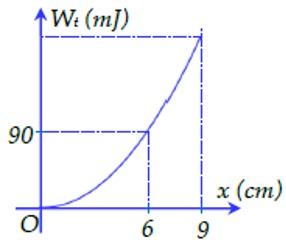
\includegraphics[scale=0.7]{../figs/G11-FINAL-SEM1-002-2}}
	\loigiai{
	$W_{\mathrm{t}}=\dfrac{1}{2}m\omega^2x^2\Rightarrow m\omega^2=50$.\\
	$W_{\mathrm{t}\max}=\dfrac{1}{2}m\omega A^2=\dfrac{1}{2}\cdot50\cdot0,09^2=\SI{202.5}{\milli\joule}$.
	}
\end{ex}
% ===================================================================
\begin{ex}
Phát biểu nào sau đây đúng khi nói về sóng cơ học?	
	\choice
	{Sóng ngang là sóng có phương dao động trùng với phương truyền sóng}
	{Sóng dọc là sóng có phương dao động vuông góc với phương truyền sóng}
	{\True Sóng dọc là sóng có phương dao động trùng với phương truyền sóng}
	{Sóng âm truyền được trong chân không}
	\loigiai{}
\end{ex}
\Closesolutionfile{ans}
\section{Câu trắc nghiệm đúng/sai} 
\textit{Thí sinh trả lời từ câu 1 đến câu 4. Trong mỗi ý \textbf{a)}, \textbf{b)}, \textbf{c)}, \textbf{d)} ở mỗi câu, thí sinh chọn đúng hoặc sai}
\setcounter{ex}{0}\\
\Opensolutionfile{ans}[ans/G11-FINAL-SEM1-002-TF]
% ===================================================================
\begin{ex}
Trên một sợi dây đàn hồi với hai đầu cố định đang có sóng dừng với bước sóng $\SI{2}{\centi\meter}$.
	\choiceTF[t]
	{\True Chiều dài sợi dây có thể nhận giá trị $\SI{9}{\centi\meter}$}
	{Khoảng cách ngắn nhát giữa một nút và một bụng là $\SI{1}{\centi\meter}$}
	{Giả sử sợi dây có chiều dài $\ell$. Trên dây đang có sóng dừng với $n$ bụng sóng, tốc độ truyền sóng trên dây là $v$. Khoảng thời gian giữa hai lần liên tiếp sợi dây duỗi thẳng là $\dfrac{\ell}{2nv}$}
	{Khi sợi dây duỗi thẳng thì tỉ số giữa chiều dài sợi dây và bước sóng bằng $n+0,5\ \left(n=1; 2; 3; \dots\right)$}
	\loigiai{}
\end{ex}
% ===================================================================
\begin{ex}
Trong thí nghiệm Young về giao thoa ánh sáng, người ta dùng nguồn sáng đơn sắc có bước sóng $\lambda=\SI{0.6}{\micro\meter}$, khoảng cách từ màn tới hai khe là $\SI{2}{\meter}$, khoảng cách giữa hai khe là $a=\SI{1}{\milli\meter}$.
	\choiceTF[t]
	{\True Tại vị trí trung tâm của trường giao thoa là vân sáng bậc 0}
	{Khoảng vân giao thoa là $i=\SI{1.2}{\centi\meter}$}
	{Vị trí cách vân sáng trung tâm $x=\SI{2.4}{\milli\meter}$ là vân sáng bậc 3}
	{\True Vị trí cách vân trung tâm $x=\SI{3}{\milli\meter}$ là vân tối thứ 3}
	\loigiai{}
\end{ex}
% ===================================================================
\begin{ex}
\immini{Một sóng cơ hình sin lan truyền trên một sợi dây đàn hồi với tần số $\SI{20}{\hertz}$. Tại thời điểm $t$, một đoạn của sợi dây có dạng như hình bên, phần tử ở P đang tạm dừng còn các phần tử ở M và N đang đi từ vị trí cân bằng của nó đi lên. Biết khoảng cách từ M đến P theo phương truyền sóng là $\SI{30}{\centi\meter}$.}
{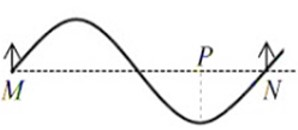
\includegraphics[scale=0.7]{../figs/G11-FINAL-SEM1-002-3}}
	\choiceTF[t]
	{\True Sóng truyền từ N đến M}
	{\True Tốc độ truyền sóng là $\SI{8}{\meter/\second}$}
	{\True Điểm Q là trung điểm của MP đang đi xuống}
	{Sau $\SI{0.025}{\second}$ thì điểm M đang đi lên}
	\loigiai{}
\end{ex}
% ===================================================================
\begin{ex}
\immini{Hệ thống treo ô tô như hình bên là ứng dụng của lò xo trong việc giảm xóc. Biết độ cứng của lò xo là $k=\SI{75}{\kilo\newton/\meter}$. Và một xe ô tô có bốn lò xo như vậy. Khi xe đứng yên mỗi lò xo bị nén $\SI{5}{\centi\meter}$. Lấy $g=\SI{10}{\meter/\second^2}$ và $\pi^2=10$. Xét tính đúng/sai của các phát biểu sau:}
{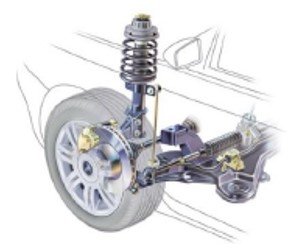
\includegraphics[scale=0.6]{../figs/G11-FINAL-SEM1-002-4}}
	\choiceTF[t]
	{Độ cứng của hệ bốn lò xo mắc song song là $\SI{18750}{\newton/\meter}$}
	{\True Phần khối lượng đè lên hệ lò xo là $\SI{1500}{\kilogram}$}
	{Nếu coi cả hệ như một con lắc lò xo dao động thì tần số dao động riêng là $\SI{5}{\hertz}$}
	{\True Hệ có khả năng giảm xóc dựa trên hiện tượng dao động tắt dần}
	\loigiai{}
\end{ex}
\Closesolutionfile{ans}
\section{Câu trắc nghiệm trả lời ngắn} \textit{Thí sinh trả lời từ câu 1 đến câu 6}
\setcounter{ex}{0}
\Opensolutionfile{ans}[ans/G11-FINAL-SEM1-002-TL]
% ===============================================================
\begin{ex}
Tại một nơi trên mặt đất, một con lắc đơn dao động điều hòa. Trong khoảng thời gian $\Delta t$, con lắc thực hiện 60 dao động toàn phần; thay đổi chiều dài con lắc một đoạn $\SI{44}{\centi\meter}$ thì cũng trong khoảng thời gian $\Delta t$ ấy, nó thực hiện 50 dao động toàn phần. Chiều dài ban đầu của con lắc là bao nhiêu $\si{\centi\meter}$? 
	\shortans[oly]{100}
	\loigiai{
		$\dfrac{\ell'}{\ell}=\left(\dfrac{T'}{T}\right)^2=\left(\dfrac{N}{N'}\right)^2\Rightarrow \dfrac{\ell+44}{\ell}=\dfrac{60}{50}\Rightarrow \ell=\SI{100}{\centi\meter}.$
	}
\end{ex}
% ===============================================================
\begin{ex}
Trong thí nghiệm Young về giao thoa ánh sáng, trong khoảng rộng $\SI{2.5}{\milli\meter}$ trên màn có 3 vân tối biết một đầu là vân tối còn một đầu là vân sáng. Biết bề rộng trường giao thoa $\SI{8.1}{\milli\meter}$. Tổng số vân sáng và vân tối có trong miền giao thoa là bao nhiêu?
	\shortans[oly]{17}
	\loigiai{
		$2,5i=2\SI{2.5}{\milli\meter}\Rightarrow i=\SI{1}{\milli\meter}$.\\
		$\dfrac{-L}{2i}\le k_s\le \dfrac{L}{2i}\Rightarrow -4,05\le k_s\le 4,05\Rightarrow N_s=9$.
		$\dfrac{-L}{2i}-0,5\le k_t\le \dfrac{L}{2i}-0,5\Rightarrow -4,55\le k_s\le 3,55\Rightarrow N_t=8$.
		Vậy tổng số vân tối và vân sáng trên màn quan sát: $N=N_s+N_t=17$.
	}
\end{ex}
% ===============================================================
\begin{ex}
Trong thí nghiệm Young về giao thoa ánh sáng, hai khe được chiếu bằng ánh sáng đơn sắc, khoảng cách giữa hai khe là $\SI{0.6}{\milli\meter}$. Khoảng vân trên màn quan sát đo được là $\SI{1}{\milli\meter}$. Từ vị trí ban đầu, nếu tịnh tiến màn quan sát một đoạn $\SI{25}{\centi\meter}$ lại gần mặt phẳng chứa hai khe thì khoảng vân mới trên màn là $\SI{0.75}{\milli\meter}$. Bước sóng của ánh sáng dùng trong thí nghiệm là bao nhiêu $\si{\micro\meter}$? 
	\shortans[oly]{0,6}
	\loigiai{
		$\Delta i=\dfrac{\lambda\Delta D}{a}\Rightarrow \lambda=\SI{0.6}{\micro\meter}$.
	}
\end{ex}
% ===============================================================
\begin{ex}
\immini{Một chất điểm dao động điều hòa, có đồ thị của li độ phụ thuộc vào thời gian như hình vẽ. Tần số dao động của vật là bao nhiêu $\si{\hertz}$?}
{\vspace{-0.75cm}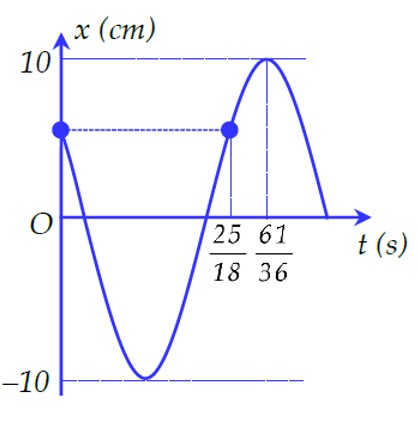
\includegraphics[scale=0.6]{../figs/G11-FINAL-SEM1-002-5}}
	\shortans[oly]{0,5}
	\loigiai{
		$T=\dfrac{61}{36}+\dfrac{61}{36}-\dfrac{25}{18}=\SI{2}{\second}$.\\
		$f=\dfrac{1}{T}=\SI{0.5}{\hertz}$.
	}
\end{ex}
% ===============================================================
\begin{ex}
	\immini{Một sóng hình sin có biên độ không đổi truyền trên một sợi dây đàn hồi rất dài với tần số là $\SI{10}{\hertz}$. Ở thời điểm $t$, hình dạng của đoạn đây như hình vẽ. Các vị trí cân bằng của các phần tử trên dây cùng nằm trên trục $Ox$. Tốc độ truyền sóng trên dây bằng bao nhiêu $\si{\centi\meter/\second}$?}
	{\vspace{-0.75cm}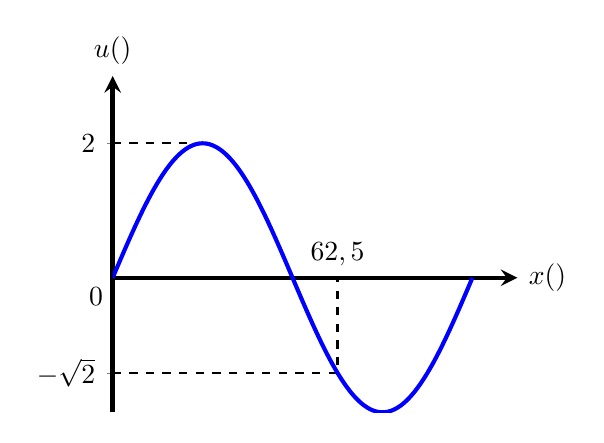
\begin{tikzpicture}  
			\begin{axis}[  ultra thick,scale=0.75,
				xmin=0,  
				xmax=9,  
				ytick={-1.4142,0,2},
				ymin=-2,  
				ymax=3, 
				samples=300,
				xtick=\empty,
				yticklabels={$-\sqrt{2}$,0,2},
				axis lines=center, 
				xlabel=$\xsi{x}{\left(\centi\meter\right)}$, 		ylabel=$\xsi{u}{\left(\si{\centi\meter}\right)}$,
				every axis y label/.style={at=(current axis.above origin),anchor=south},  
				every axis x label/.style={at=(current axis.right of origin),anchor=west},  ]
				\draw[line width=0.8pt, dashed] (0,-1.4142)--(5,-1.4142)--(5,0);
				\draw[line width=0.8pt, dashed] (0,2)--(2,2);
				\addplot [line width=1.5pt, blue, smooth, domain=0:8] {2*cos(deg(pi*x/4-0.5*pi))};  
				\coordinate (O) at (axis cs: 0,0);
				\node[above] at (axis cs: 5,0)  {$62,5$};
			\end{axis}  
			\node[below left] at (O) {0};
	\end{tikzpicture}}
	\shortans[oly]{1000}
	\loigiai{
		$\dfrac{2\pi x}{\lambda}=\pi+\dfrac{\pi}{4}\Rightarrow \lambda=\dfrac{8x}{5}=\dfrac{8\cdot62,5}{5}=\SI{100}{\centi\meter}$.\\
		$v=\lambda f=\SI{1000}{\centi\meter/\second}$.
	}
\end{ex}
% ===============================================================
\begin{ex}
\immini{Trong hiện tượng sóng dừng, xảy ra trên một sợi dây đàn hồi OB. Đồ thị bên là hình ảnh sợi dây tại hai thời điểm $t_1$ và $t_2=t_1+\xsi{\dfrac{1}{3}}{\second}$ (ngay sau đó). Biết rằng tại thời điểm $t_1$, điểm M có vận tốc bằng 0. Tốc độ truyền sóng trên dây bằng bao nhiêu $\si{\centi\meter/\second}$?}
{\vspace{-0.75cm}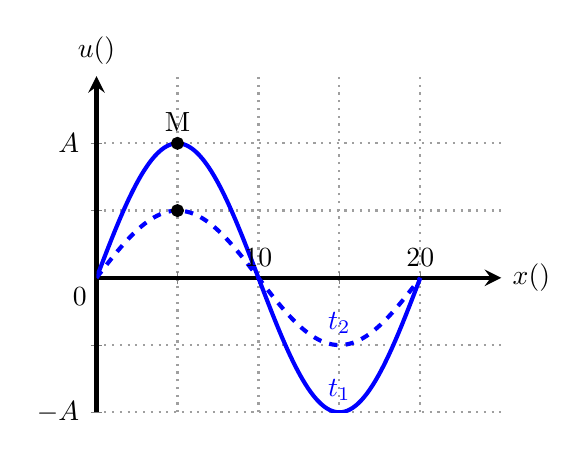
\begin{tikzpicture}  
		\begin{axis}[  ultra thick,scale=0.75,
			xmin=0,  
			xmax=5,  
			xtick={0,1,...,4},
			ytick={-2,-1,1,2},
			ymin=-2,  
			ymax=3, 
			samples=300,
			yticklabels={$-A$,,, $A$},
			xticklabels=\empty,
			axis lines=center, 
			grid style={step=1, line width =0.4pt, color=gray!40!white},
			grid=both, %giới hạn ô lưới
			major grid style={line width=0.8pt,gray!75!white, dotted},
			xlabel=$\xsi{x}{\left(\centi\meter\right)}$, 		ylabel=$\xsi{u}{\left(\si{\centi\meter}\right)}$,
			every axis y label/.style={at=(current axis.above origin),anchor=south},  
			every axis x label/.style={at=(current axis.right of origin),anchor=west},  ]
			\addplot [line width=1.5pt, blue, smooth, domain=0:4] {2*cos(deg(pi*x/2-0.5*pi))} node[above] at(axis cs:3,-2) {$t_1$};  
			\addplot [line width=1.5pt, blue, dashed,smooth, domain=0:4] {1*cos(deg(pi*x/2-0.5*pi))} node[above] at(axis cs:3,-1) {$t_2$};
			\filldraw (axis cs: 1,2) circle(1.5pt) node[above]{M};
			\filldraw (axis cs: 1,1) circle(1.5pt);
			\coordinate (O) at (axis cs: 0,0);
			\node[above] at(axis cs:2,0) {10};
			\node[above] at(axis cs:4,0) {20};
		\end{axis}  
		\node[below left] at (O) {0};
\end{tikzpicture}}
	\shortans[oly]{10}
	\loigiai{
		$t_2-t_1=\dfrac{T}{6}=\xsi{\dfrac{1}{3}}{\second}\Rightarrow T=\SI{2}{\second}$.\\
		$v=\dfrac{\lambda}{T}=\SI{10}{\centi\meter/\second}$.
	}
\end{ex}
\Closesolutionfile{ans}
\begin{center}
	\textbf{--- HẾT ---}
\end{center}